%%
%% ****** ljmsamp.tex 13.06.2018 ******
%%
\documentclass[
11pt,%
tightenlines,%
twoside,%
onecolumn,%
nofloats,%
nobibnotes,%
nofootinbib,%
superscriptaddress,%
noshowpacs,%
centertags]%
{revtex4}
\usepackage{ljm}
\begin{document}

\titlerunning{Vectorization with AVX-512 instructions} % for running heads
\authorrunning{A.~A.~Rybakov and S.~S.~Shumilin} % for running heads
%\authorrunning{First-Author, Second-Author} % for running heads

\title{Vectorization of High-performance Scientific Calculations\\
Using AVX-512 Intruction Set}
% Splitting into lines is performed by the command \\
% The title is written in accordance with the rules of capitalization.

\author{\firstname{A.~A.}~\surname{Rybakov}}
\email[E-mail: ]{rybakov.aax@gmail.com}
\affiliation{Joint Supercomputer Center of the Russian Academy of Sciences - branch of Scientific Research Institute of System Analysis of the Russian Academy of Sciences, Leninsky prospect 32a, Moscow, 119334, Russia}

\author{\firstname{S.~S.}~\surname{Shumilin}}
\email[E-mail: ]{shumilin@jscc.ru}
\affiliation{Joint Supercomputer Center of the Russian Academy of Sciences - branch of Scientific Research Institute of System Analysis of the Russian Academy of Sciences, Leninsky prospect 32a, Moscow, 119334, Russia}
%\noaffiliation % If the author does not specify a place of work.

\firstcollaboration{(Submitted by G.~I.~Savin)} % Add if you know submitter.
%\lastcollaboration{ }

\received{June 13, 2018} % The date of receipt to the editor, i.e. December 06, 2017


\begin{abstract} % You shouldn't use formulas and citations in the abstract.
The man in black fled across the desert, and the gunslinger followed. The desert was the apotheosis of all deserts, huge, standing to the sky for what might have been parsecs in all directions. White; blinding; waterless; without feature save for the faint, cloudy haze of the mountains which sketched themselves on the horizon and the devil-grass which brought sweet dreams, nightmares, death. An occasional tombstone sign pointed the way, for once the drifted track that cut its way through the thick crust of alkali had been a highway and coaches had followed it. The world had moved on since then. The world had emptied.
\end{abstract}

\subclass{68N19} % Enter 2010 Mathematics Subject Classification.

\keywords{Optimization, vectorization, AVX-512, predicated execution, intrinsics, application performance.} % Include keywords separeted by comma.

\maketitle

% Text of article starts here.

\section{Introduction}

The gunslinger walked stolidly, not hurrying, not loafing. A hide waterbag was slung around his middle like a bloated sausage. It was almost full. He had progressed through the khef over many years, and had reached the fifth level. At the seventh or eighth, he would not have been thirsty; he could have watched own body dehydrate with clinical, detached attention, watering its crevices and dark inner hollows only when his logic told him it must be done. He was not seventh or eighth. He was fifth. So he was thirsty, although he had no particular urge to drink. In a vague way, all this pleased him. It was romantic.

Below the waterbag were his guns, finely weighted to his hand. The two belts crisscrossed above his crotch. The holsters were oiled too deeply for even this Philistine sun to crack. The stocks of the guns were sandalwood, yellow and finely grained. The holsters were tied down with raw hide cord, and they swung heavily against his hips. The brass casings of the cartridges looped into the gun belts twinkled and flashed and heliographed in the sun. The leather made subtle creaking noises. The guns themselves made no noise. They had spilled blood. There was no need to make noise in the sterility of the desert.

\begin{table}[!h]
\setcaptionmargin{0mm}
\onelinecaptionsfalse
\captionstyle{flushleft}
\caption{ For the insertion of tables, the table environment is used,
 the signatures to the tables are made in the same way as the captions
 for the figures. This is an example of a table whose multi-line name
 is decorated with the \textbf{caption2} package.}
\bigskip
\begin{tabular}{|c|c|c|c|c|c|c|c|}
\hline
 &$r_c$ (\AA)&$r_0$ (\AA)&$\kappa r_0$&
 &$r_c$ (\AA) &$r_0$ (\AA)&$\kappa r_0$\\
\hline
Cu& 0.800 & 14.10 & 2.550 &Sn
& 0.680 & 1.870 & 3.700 \\
Ag& 0.990 & 15.90 & 2.710 &Pb
& 0.450 & 1.930 & 3.760 \\
Au& 1.150 & 15.90 & 2.710 &Ca
& 0.750 & 2.170 & 3.560 \\
Mg& 0.490 & 17.60 & 3.200 &Sr
& 0.900 & 2.370 & 3.720 \\
Zn& 0.300 & 15.20 & 2.970 &Li
& 0.380 & 1.730 & 2.830 \\
Cd& 0.530 & 17.10 & 3.160 &Na
& 0.760 & 2.110 & 3.120 \\
Hg& 0.550 & 17.80 & 3.220 &K &  1.120 & 2.620 & 3.480 \\
Al& 0.230 & 15.80 & 3.240 &Rb & 1.330 & 2.800 & 3.590 \\
Ga& 0.310 & 16.70 & 3.330 &Cs & 1.420 & 3.030 & 3.740 \\
In& 0.460 & 18.40 & 3.500 &Ba & 0.960 & 2.460 & 3.780 \\
Tl& 0.480 & 18.90 & 3.550 & & & & \\[1mm]
\hline
\end{tabular}
\end{table}

His clothes were the no-color of rain or dust. His shirt was open at the throat, with a rawhide thong dangling loosely in hand-punched eyelets. His pants were seam-stretched dungarees.

He breasted a gently rising dune (although there was no sand here; the desert was hardpan, and even the harsh winds that blew when dark came raised only an aggravating harsh dust like scouring powder) and saw the kicked remains of a tiny campfire on the lee side, the side which the sun would quit earliest. Small signs like this, once more affirming the man in black?s essential humanity, never failed to please him. His lips stretched in the pitted, flaked remains of his face. He squatted.

He had burned the devil-grass, of course. It was the only thing out here that would burn. It burned with a greasy, flat light, and it burned slow. Border dwellers had told him that devils lived even in the flames. They burned it but would not look into the light. They said the devils hypnotized, beckoned, would eventually draw the one who looked into the fires. And the next man foolish enough to look into the fire might see you.

The burned grass was crisscrossed in the now-familiar ideographic pattern, and crumbled to gray senselessness before the gunslinger?s prodding hand. 

There was nothing in the remains but a charred scrap of bacon, which he ate thoughtfully. It had always been this way. The gunslinger had followed the man in black across the desert for two months now, across the endless, screamingly monotonous purgatorial wastes, and had yet to find spoor other than the hygienic sterile ideographs of the man in black?s camp fires. He had not found a can, a bottle, or a waterbag (the gunslinger had left four of those behind, like dead snake-skins).

\section{First level Heading}

The gunslinger walked stolidly, not hurrying, not loafing. A hide waterbag was slung around his middle like a bloated sausage. It was almost full. He had progressed through the khef over many years, and had reached the fifth level. At the seventh or eighth, he would not have been thirsty; he could have watched own body dehydrate with clinical, detached attention, watering its crevices and dark inner hollows only when his logic told him it must be done. He was not seventh or eighth. He was fifth. So he was thirsty, although he had no particular urge to drink. In a vague way, all this pleased him. It was romantic.

\begin{figure}[h]
\setcaptionmargin{5mm}
%\onelinecaptionsfalse % if the caption is multiline
\onelinecaptionstrue  % if the caption is one-line
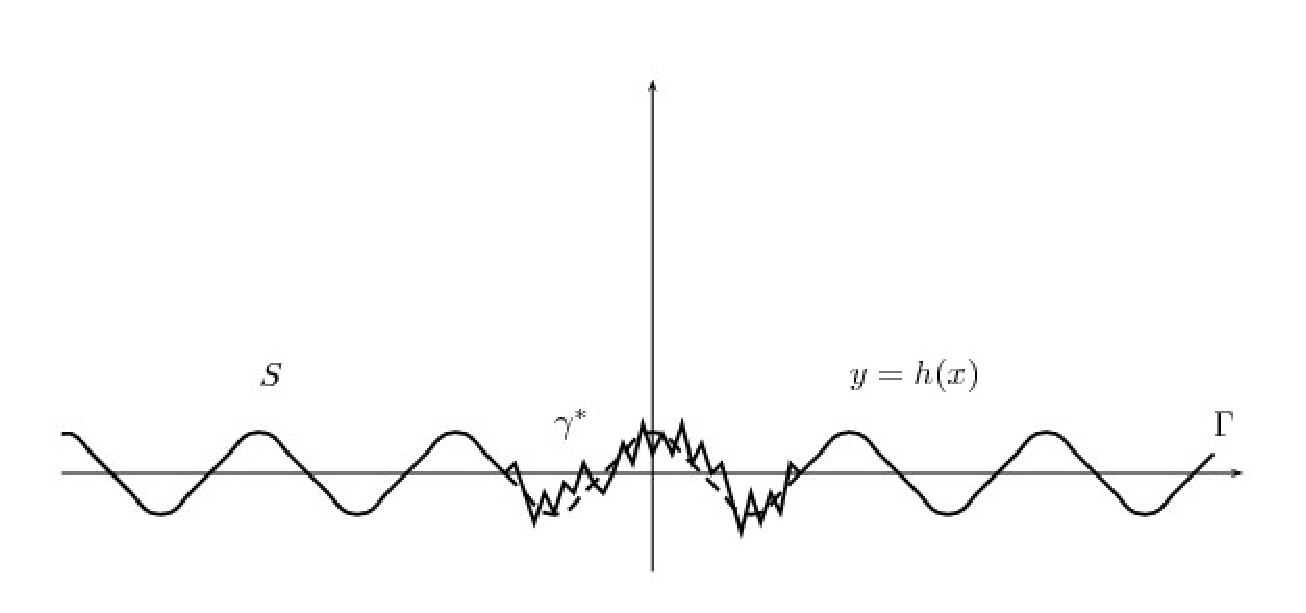
\includegraphics[width=0.85\textwidth]{deform.eps}
\captionstyle{normal}\caption{Please write your figure caption here.}\label{fig:1}
\end{figure}

Below the waterbag were his guns, finely weighted to his hand. The two belts crisscrossed above his crotch. The holsters were oiled too deeply for even this Philistine sun to crack. The stocks of the guns were sandalwood, yellow and finely grained. The holsters were tied down with raw hide cord, and they swung heavily against his hips. The brass casings of the cartridges looped into the gun belts twinkled and flashed and heliographed in the sun. The leather made subtle creaking noises. The guns themselves made no noise. They had spilled blood. There was no need to make noise in the sterility of the desert.

\begin{multline}
\int_{a_1}^{a_2} f(x)\,dx+\int_{a_2}^{a_3} f(x)\,dx
+\dots+\int_{a_{n-1}}^{a_n} f(x)\,dx\\
+\int_{a_1}^{a_2} g(x)\,dx+\int_{a_2}^{a_3} g(x)\,dx
+\dots+\int_{a_{n-1}}^{a_n} g(x)\,dx\\
+\int_{a_1}^{a_2} h(x)\,dx+\int_{a_2}^{a_3} h(x)\,dx
+\dots+\int_{a_{n-1}}^{a_n} h(x)\,dx\\
=\int_{a_1}^{a_n} f(x)+g(x)+h(x)\,dx.
\end{multline}

His clothes were the no-color of rain or dust. His shirt was open at the throat, with a rawhide thong dangling loosely in hand-punched eyelets. His pants were seam-stretched dungarees.

He breasted a gently rising dune (although there was no sand here; the desert was hardpan, and even the harsh winds that blew when dark came raised only an aggravating harsh dust like scouring powder) and saw the kicked remains of a tiny campfire on the lee side, the side which the sun would quit earliest. Small signs like this, once more affirming the man in black?s essential humanity, never failed to please him. His lips stretched in the pitted, flaked remains of his face. He squatted.

\begin{figure}[h]
\setcaptionmargin{5mm}
%\onelinecaptionsfalse % if the caption is multiline
\onelinecaptionstrue  % if the caption is one-line
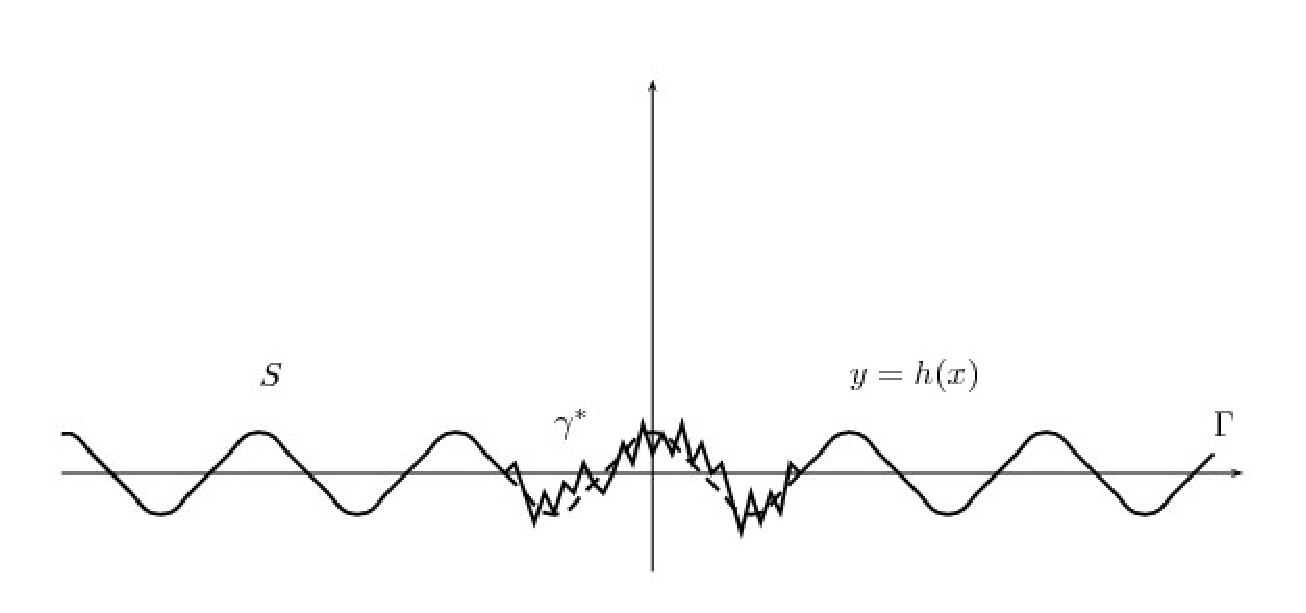
\includegraphics[width=0.85\textwidth]{deform.eps}
\captionstyle{normal}\caption{Please write your figure caption here.}\label{fig:1}
\end{figure}

He had burned the devil-grass, of course. It was the only thing out here that would burn. It burned with a greasy, flat light, and it burned slow. Border dwellers had told him that devils lived even in the flames. They burned it but would not look into the light. They said the devils hypnotized, beckoned, would eventually draw the one who looked into the fires. And the next man foolish enough to look into the fire might see you.

The burned grass was crisscrossed in the now-familiar ideographic pattern, and crumbled to gray senselessness before the gunslinger?s prodding hand. 

There was nothing in the remains but a charred scrap of bacon, which he ate thoughtfully. It had always been this way. The gunslinger had followed the man in black across the desert for two months now, across the endless, screamingly monotonous purgatorial wastes, and had yet to find spoor other than the hygienic sterile ideographs of the man in black?s camp fires. He had not found a can, a bottle, or a waterbag (the gunslinger had left four of those behind, like dead snake-skins).

The gunslinger walked stolidly, not hurrying, not loafing. A hide waterbag was slung around his middle like a bloated sausage. It was almost full. He had progressed through the khef over many years, and had reached the fifth level. At the seventh or eighth, he would not have been thirsty; he could have watched own body dehydrate with clinical, detached attention, watering its crevices and dark inner hollows only when his logic told him it must be done. He was not seventh or eighth. He was fifth. So he was thirsty, although he had no particular urge to drink. In a vague way, all this pleased him. It was romantic.

Below the waterbag were his guns, finely weighted to his hand. The two belts crisscrossed above his crotch. The holsters were oiled too deeply for even this Philistine sun to crack. The stocks of the guns were sandalwood, yellow and finely grained. The holsters were tied down with raw hide cord, and they swung heavily against his hips. The brass casings of the cartridges looped into the gun belts twinkled and flashed and heliographed in the sun. The leather made subtle creaking noises. The guns themselves made no noise. They had spilled blood. There was no need to make noise in the sterility of the desert.

His clothes were the no-color of rain or dust. His shirt was open at the throat, with a rawhide thong dangling loosely in hand-punched eyelets. His pants were seam-stretched dungarees.

He breasted a gently rising dune (although there was no sand here; the desert was hardpan, and even the harsh winds that blew when dark came raised only an aggravating harsh dust like scouring powder) and saw the kicked remains of a tiny campfire on the lee side, the side which the sun would quit earliest. Small signs like this, once more affirming the man in black?s essential humanity, never failed to please him. His lips stretched in the pitted, flaked remains of his face. He squatted.

He had burned the devil-grass, of course. It was the only thing out here that would burn. It burned with a greasy, flat light, and it burned slow. Border dwellers had told him that devils lived even in the flames. They burned it but would not look into the light. They said the devils hypnotized, beckoned, would eventually draw the one who looked into the fires. And the next man foolish enough to look into the fire might see you.

The burned grass was crisscrossed in the now-familiar ideographic pattern, and crumbled to gray senselessness before the gunslinger?s prodding hand. 

There was nothing in the remains but a charred scrap of bacon, which he ate thoughtfully. It had always been this way. The gunslinger had followed the man in black across the desert for two months now, across the endless, screamingly monotonous purgatorial wastes, and had yet to find spoor other than the hygienic sterile ideographs of the man in black?s camp fires. He had not found a can, a bottle, or a waterbag (the gunslinger had left four of those behind, like dead snake-skins).

\section{Standalone formulae}

The gunslinger walked stolidly, not hurrying, not loafing. A hide waterbag was slung around his middle like a bloated sausage. It was almost full. He had progressed through the khef over many years, and had reached the fifth level. At the seventh or eighth, he would not have been thirsty; he could have watched own body dehydrate with clinical, detached attention, watering its crevices and dark inner hollows only when his logic told him it must be done. He was not seventh or eighth. He was fifth. So he was thirsty, although he had no particular urge to drink. In a vague way, all this pleased him. It was romantic.

\begin{figure}[h]
\setcaptionmargin{5mm}
%\onelinecaptionsfalse % if the caption is multiline
\onelinecaptionstrue  % if the caption is one-line
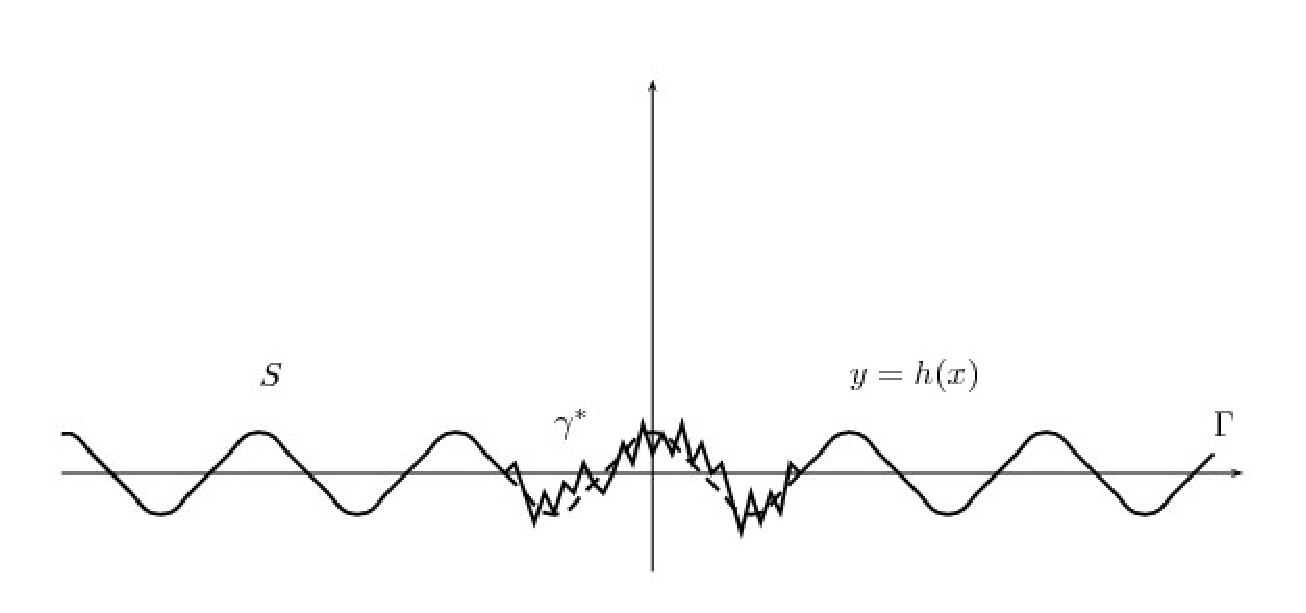
\includegraphics[width=0.85\textwidth]{deform.eps}
\captionstyle{normal}\caption{Please write your figure caption here.}\label{fig:1}
\end{figure}

Below the waterbag were his guns, finely weighted to his hand. The two belts crisscrossed above his crotch. The holsters were oiled too deeply for even this Philistine sun to crack. The stocks of the guns were sandalwood, yellow and finely grained. The holsters were tied down with raw hide cord, and they swung heavily against his hips. The brass casings of the cartridges looped into the gun belts twinkled and flashed and heliographed in the sun. The leather made subtle creaking noises. The guns themselves made no noise. They had spilled blood. There was no need to make noise in the sterility of the desert.

His clothes were the no-color of rain or dust. His shirt was open at the throat, with a rawhide thong dangling loosely in hand-punched eyelets. His pants were seam-stretched dungarees.

He breasted a gently rising dune (although there was no sand here; the desert was hardpan, and even the harsh winds that blew when dark came raised only an aggravating harsh dust like scouring powder) and saw the kicked remains of a tiny campfire on the lee side, the side which the sun would quit earliest. Small signs like this, once more affirming the man in black?s essential humanity, never failed to please him. His lips stretched in the pitted, flaked remains of his face. He squatted.

\begin{multline}
\int_{a_1}^{a_2} f(x)\,dx+\int_{a_2}^{a_3} f(x)\,dx
+\dots+\int_{a_{n-1}}^{a_n} f(x)\,dx\\
+\int_{a_1}^{a_2} g(x)\,dx+\int_{a_2}^{a_3} g(x)\,dx
+\dots+\int_{a_{n-1}}^{a_n} g(x)\,dx\\
+\int_{a_1}^{a_2} h(x)\,dx+\int_{a_2}^{a_3} h(x)\,dx
+\dots+\int_{a_{n-1}}^{a_n} h(x)\,dx\\
=\int_{a_1}^{a_n} f(x)+g(x)+h(x)\,dx.
\end{multline}

He had burned the devil-grass, of course. It was the only thing out here that would burn. It burned with a greasy, flat light, and it burned slow. Border dwellers had told him that devils lived even in the flames. They burned it but would not look into the light. They said the devils hypnotized, beckoned, would eventually draw the one who looked into the fires. And the next man foolish enough to look into the fire might see you.

The burned grass was crisscrossed in the now-familiar ideographic pattern, and crumbled to gray senselessness before the gunslinger?s prodding hand. 

There was nothing in the remains but a charred scrap of bacon, which he ate thoughtfully. It had always been this way. The gunslinger had followed the man in black across the desert for two months now, across the endless, screamingly monotonous purgatorial wastes, and had yet to find spoor other than the hygienic sterile ideographs of the man in black?s camp fires. He had not found a can, a bottle, or a waterbag (the gunslinger had left four of those behind, like dead snake-skins).

\begin{figure}[h]
\setcaptionmargin{5mm}
%\onelinecaptionsfalse % if the caption is multiline
\onelinecaptionstrue  % if the caption is one-line
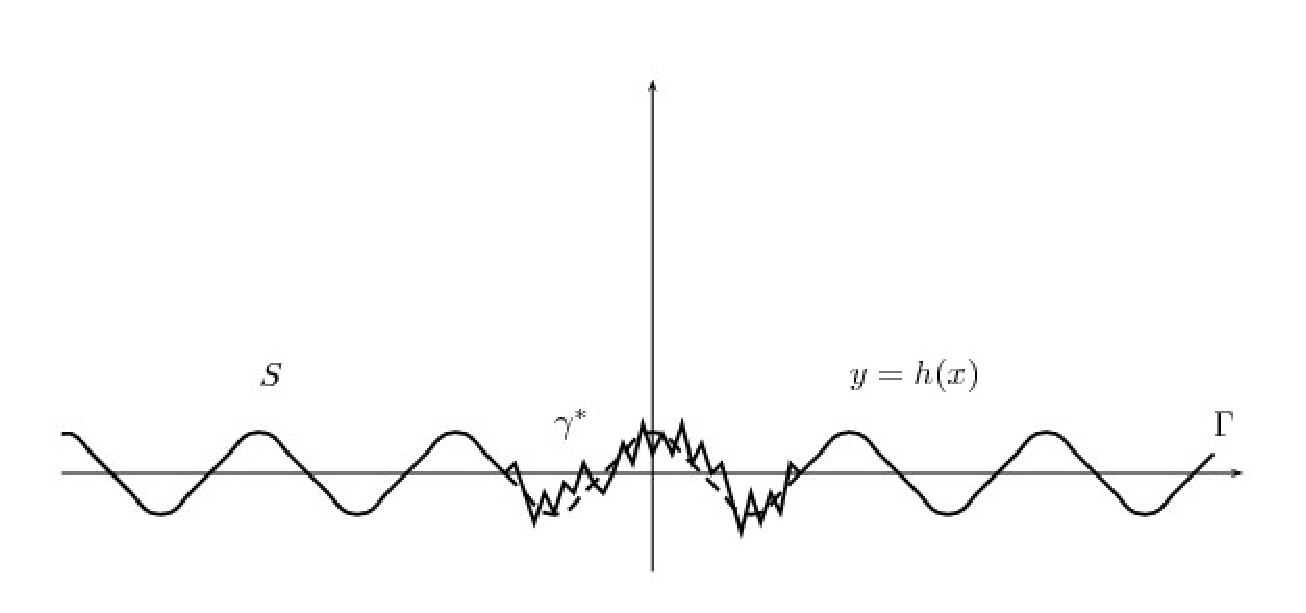
\includegraphics[width=0.85\textwidth]{deform.eps}
\captionstyle{normal}\caption{Please write your figure caption here.}\label{fig:1}
\end{figure}

The gunslinger walked stolidly, not hurrying, not loafing. A hide waterbag was slung around his middle like a bloated sausage. It was almost full. He had progressed through the khef over many years, and had reached the fifth level. At the seventh or eighth, he would not have been thirsty; he could have watched own body dehydrate with clinical, detached attention, watering its crevices and dark inner hollows only when his logic told him it must be done. He was not seventh or eighth. He was fifth. So he was thirsty, although he had no particular urge to drink. In a vague way, all this pleased him. It was romantic.

Below the waterbag were his guns, finely weighted to his hand. The two belts crisscrossed above his crotch. The holsters were oiled too deeply for even this Philistine sun to crack. The stocks of the guns were sandalwood, yellow and finely grained. The holsters were tied down with raw hide cord, and they swung heavily against his hips. The brass casings of the cartridges looped into the gun belts twinkled and flashed and heliographed in the sun. The leather made subtle creaking noises. The guns themselves made no noise. They had spilled blood. There was no need to make noise in the sterility of the desert.

His clothes were the no-color of rain or dust. His shirt was open at the throat, with a rawhide thong dangling loosely in hand-punched eyelets. His pants were seam-stretched dungarees.

He breasted a gently rising dune (although there was no sand here; the desert was hardpan, and even the harsh winds that blew when dark came raised only an aggravating harsh dust like scouring powder) and saw the kicked remains of a tiny campfire on the lee side, the side which the sun would quit earliest. Small signs like this, once more affirming the man in black?s essential humanity, never failed to please him. His lips stretched in the pitted, flaked remains of his face. He squatted.

He had burned the devil-grass, of course. It was the only thing out here that would burn. It burned with a greasy, flat light, and it burned slow. Border dwellers had told him that devils lived even in the flames. They burned it but would not look into the light. They said the devils hypnotized, beckoned, would eventually draw the one who looked into the fires. And the next man foolish enough to look into the fire might see you.

The burned grass was crisscrossed in the now-familiar ideographic pattern, and crumbled to gray senselessness before the gunslinger?s prodding hand. 

There was nothing in the remains but a charred scrap of bacon, which he ate thoughtfully. It had always been this way. The gunslinger had followed the man in black across the desert for two months now, across the endless, screamingly monotonous purgatorial wastes, and had yet to find spoor other than the hygienic sterile ideographs of the man in black?s camp fires. He had not found a can, a bottle, or a waterbag (the gunslinger had left four of those behind, like dead snake-skins).

\section{Variables}

The gunslinger walked stolidly, not hurrying, not loafing. A hide waterbag was slung around his middle like a bloated sausage. It was almost full. He had progressed through the khef over many years, and had reached the fifth level. At the seventh or eighth, he would not have been thirsty; he could have watched own body dehydrate with clinical, detached attention, watering its crevices and dark inner hollows only when his logic told him it must be done. He was not seventh or eighth. He was fifth. So he was thirsty, although he had no particular urge to drink. In a vague way, all this pleased him. It was romantic.

Below the waterbag were his guns, finely weighted to his hand. The two belts crisscrossed above his crotch. The holsters were oiled too deeply for even this Philistine sun to crack. The stocks of the guns were sandalwood, yellow and finely grained. The holsters were tied down with raw hide cord, and they swung heavily against his hips. The brass casings of the cartridges looped into the gun belts twinkled and flashed and heliographed in the sun. The leather made subtle creaking noises. The guns themselves made no noise. They had spilled blood. There was no need to make noise in the sterility of the desert.

\begin{figure}[h]
\setcaptionmargin{5mm}
%\onelinecaptionsfalse % if the caption is multiline
\onelinecaptionstrue  % if the caption is one-line
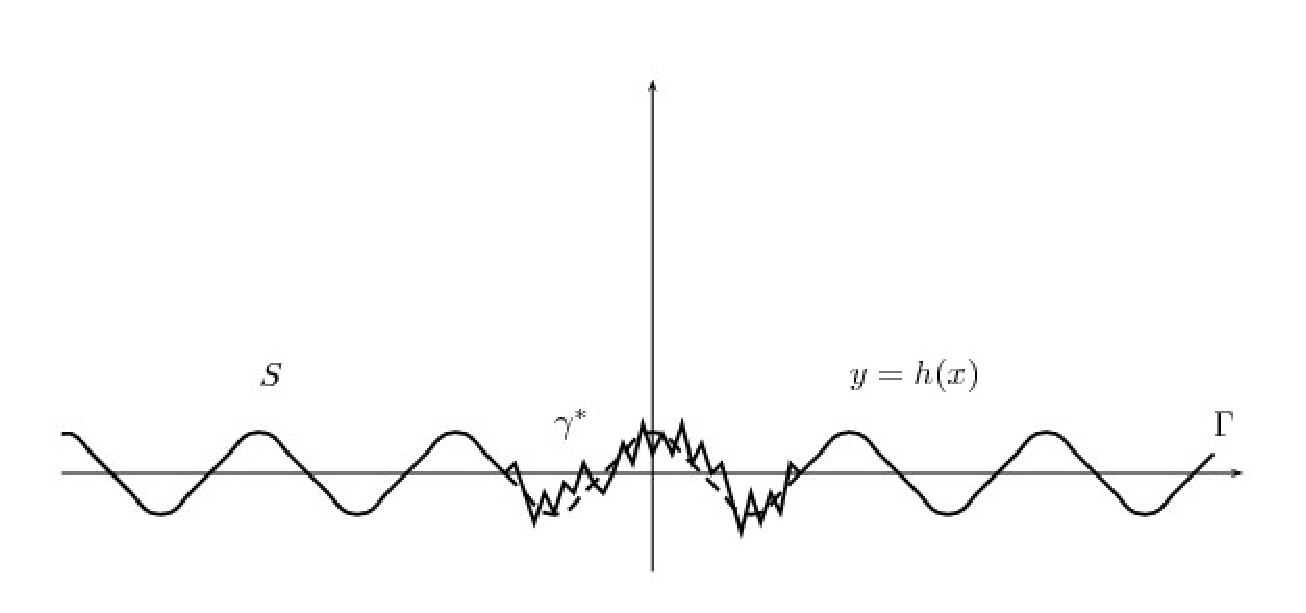
\includegraphics[width=0.85\textwidth]{deform.eps}
\captionstyle{normal}\caption{Please write your figure caption here.}\label{fig:1}
\end{figure}

His clothes were the no-color of rain or dust. His shirt was open at the throat, with a rawhide thong dangling loosely in hand-punched eyelets. His pants were seam-stretched dungarees.

He breasted a gently rising dune (although there was no sand here; the desert was hardpan, and even the harsh winds that blew when dark came raised only an aggravating harsh dust like scouring powder) and saw the kicked remains of a tiny campfire on the lee side, the side which the sun would quit earliest. Small signs like this, once more affirming the man in black?s essential humanity, never failed to please him. His lips stretched in the pitted, flaked remains of his face. He squatted.

He had burned the devil-grass, of course. It was the only thing out here that would burn. It burned with a greasy, flat light, and it burned slow. Border dwellers had told him that devils lived even in the flames. They burned it but would not look into the light. They said the devils hypnotized, beckoned, would eventually draw the one who looked into the fires. And the next man foolish enough to look into the fire might see you.

\begin{multline}
\int_{a_1}^{a_2} f(x)\,dx+\int_{a_2}^{a_3} f(x)\,dx
+\dots+\int_{a_{n-1}}^{a_n} f(x)\,dx\\
+\int_{a_1}^{a_2} g(x)\,dx+\int_{a_2}^{a_3} g(x)\,dx
+\dots+\int_{a_{n-1}}^{a_n} g(x)\,dx\\
+\int_{a_1}^{a_2} h(x)\,dx+\int_{a_2}^{a_3} h(x)\,dx
+\dots+\int_{a_{n-1}}^{a_n} h(x)\,dx\\
=\int_{a_1}^{a_n} f(x)+g(x)+h(x)\,dx.
\end{multline}

The burned grass was crisscrossed in the now-familiar ideographic pattern, and crumbled to gray senselessness before the gunslinger?s prodding hand. 

There was nothing in the remains but a charred scrap of bacon, which he ate thoughtfully. It had always been this way. The gunslinger had followed the man in black across the desert for two months now, across the endless, screamingly monotonous purgatorial wastes, and had yet to find spoor other than the hygienic sterile ideographs of the man in black?s camp fires. He had not found a can, a bottle, or a waterbag (the gunslinger had left four of those behind, like dead snake-skins).

The gunslinger walked stolidly, not hurrying, not loafing. A hide waterbag was slung around his middle like a bloated sausage. It was almost full. He had progressed through the khef over many years, and had reached the fifth level. At the seventh or eighth, he would not have been thirsty; he could have watched own body dehydrate with clinical, detached attention, watering its crevices and dark inner hollows only when his logic told him it must be done. He was not seventh or eighth. He was fifth. So he was thirsty, although he had no particular urge to drink. In a vague way, all this pleased him. It was romantic.

Below the waterbag were his guns, finely weighted to his hand. The two belts crisscrossed above his crotch. The holsters were oiled too deeply for even this Philistine sun to crack. The stocks of the guns were sandalwood, yellow and finely grained. The holsters were tied down with raw hide cord, and they swung heavily against his hips. The brass casings of the cartridges looped into the gun belts twinkled and flashed and heliographed in the sun. The leather made subtle creaking noises. The guns themselves made no noise. They had spilled blood. There was no need to make noise in the sterility of the desert.

His clothes were the no-color of rain or dust. His shirt was open at the throat, with a rawhide thong dangling loosely in hand-punched eyelets. His pants were seam-stretched dungarees.

He breasted a gently rising dune (although there was no sand here; the desert was hardpan, and even the harsh winds that blew when dark came raised only an aggravating harsh dust like scouring powder) and saw the kicked remains of a tiny campfire on the lee side, the side which the sun would quit earliest. Small signs like this, once more affirming the man in black?s essential humanity, never failed to please him. His lips stretched in the pitted, flaked remains of his face. He squatted.

He had burned the devil-grass, of course. It was the only thing out here that would burn. It burned with a greasy, flat light, and it burned slow. Border dwellers had told him that devils lived even in the flames. They burned it but would not look into the light. They said the devils hypnotized, beckoned, would eventually draw the one who looked into the fires. And the next man foolish enough to look into the fire might see you.

\begin{figure}[h]
\setcaptionmargin{5mm}
%\onelinecaptionsfalse % if the caption is multiline
\onelinecaptionstrue  % if the caption is one-line
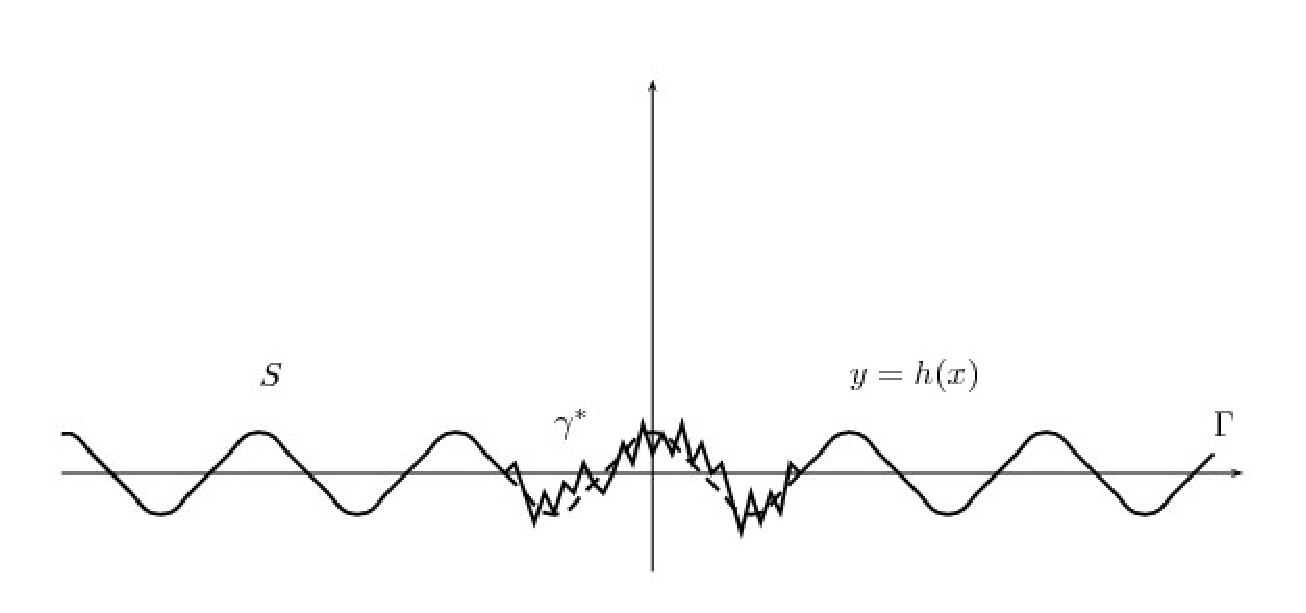
\includegraphics[width=0.85\textwidth]{deform.eps}
\captionstyle{normal}\caption{Please write your figure caption here.}\label{fig:1}
\end{figure}

The burned grass was crisscrossed in the now-familiar ideographic pattern, and crumbled to gray senselessness before the gunslinger?s prodding hand. 

There was nothing in the remains but a charred scrap of bacon, which he ate thoughtfully. It had always been this way. The gunslinger had followed the man in black across the desert for two months now, across the endless, screamingly monotonous purgatorial wastes, and had yet to find spoor other than the hygienic sterile ideographs of the man in black?s camp fires. He had not found a can, a bottle, or a waterbag (the gunslinger had left four of those behind, like dead snake-skins).

\section{Variables}

The gunslinger walked stolidly, not hurrying, not loafing. A hide waterbag was slung around his middle like a bloated sausage. It was almost full. He had progressed through the khef over many years, and had reached the fifth level. At the seventh or eighth, he would not have been thirsty; he could have watched own body dehydrate with clinical, detached attention, watering its crevices and dark inner hollows only when his logic told him it must be done. He was not seventh or eighth. He was fifth. So he was thirsty, although he had no particular urge to drink. In a vague way, all this pleased him. It was romantic.

Below the waterbag were his guns, finely weighted to his hand. The two belts crisscrossed above his crotch. The holsters were oiled too deeply for even this Philistine sun to crack. The stocks of the guns were sandalwood, yellow and finely grained. The holsters were tied down with raw hide cord, and they swung heavily against his hips. The brass casings of the cartridges looped into the gun belts twinkled and flashed and heliographed in the sun. The leather made subtle creaking noises. The guns themselves made no noise. They had spilled blood. There was no need to make noise in the sterility of the desert.

His clothes were the no-color of rain or dust. His shirt was open at the throat, with a rawhide thong dangling loosely in hand-punched eyelets. His pants were seam-stretched dungarees.

\begin{figure}[h]
\setcaptionmargin{5mm}
%\onelinecaptionsfalse % if the caption is multiline
\onelinecaptionstrue  % if the caption is one-line
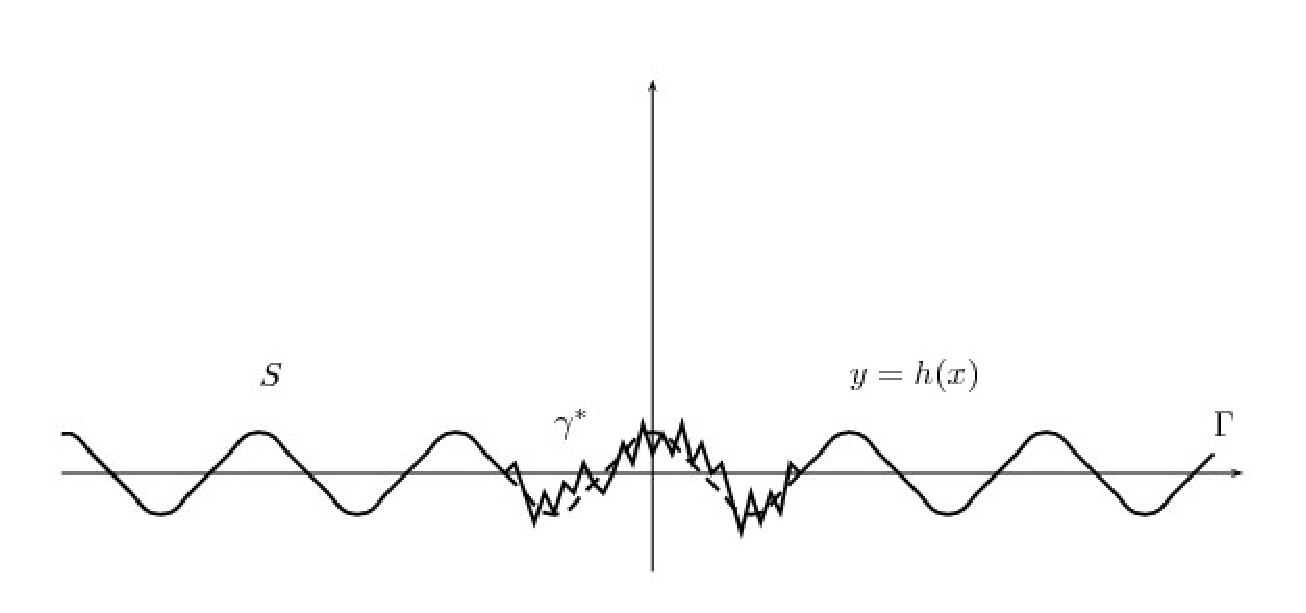
\includegraphics[width=0.85\textwidth]{deform.eps}
\captionstyle{normal}\caption{Please write your figure caption here.}\label{fig:1}
\end{figure}

He breasted a gently rising dune (although there was no sand here; the desert was hardpan, and even the harsh winds that blew when dark came raised only an aggravating harsh dust like scouring powder) and saw the kicked remains of a tiny campfire on the lee side, the side which the sun would quit earliest. Small signs like this, once more affirming the man in black?s essential humanity, never failed to please him. His lips stretched in the pitted, flaked remains of his face. He squatted.

He had burned the devil-grass, of course. It was the only thing out here that would burn. It burned with a greasy, flat light, and it burned slow. Border dwellers had told him that devils lived even in the flames. They burned it but would not look into the light. They said the devils hypnotized, beckoned, would eventually draw the one who looked into the fires. And the next man foolish enough to look into the fire might see you.

The burned grass was crisscrossed in the now-familiar ideographic pattern, and crumbled to gray senselessness before the gunslinger?s prodding hand. 

There was nothing in the remains but a charred scrap of bacon, which he ate thoughtfully. It had always been this way. The gunslinger had followed the man in black across the desert for two months now, across the endless, screamingly monotonous purgatorial wastes, and had yet to find spoor other than the hygienic sterile ideographs of the man in black?s camp fires. He had not found a can, a bottle, or a waterbag (the gunslinger had left four of those behind, like dead snake-skins).

\begin{figure}[h]
\setcaptionmargin{5mm}
%\onelinecaptionsfalse % if the caption is multiline
\onelinecaptionstrue  % if the caption is one-line
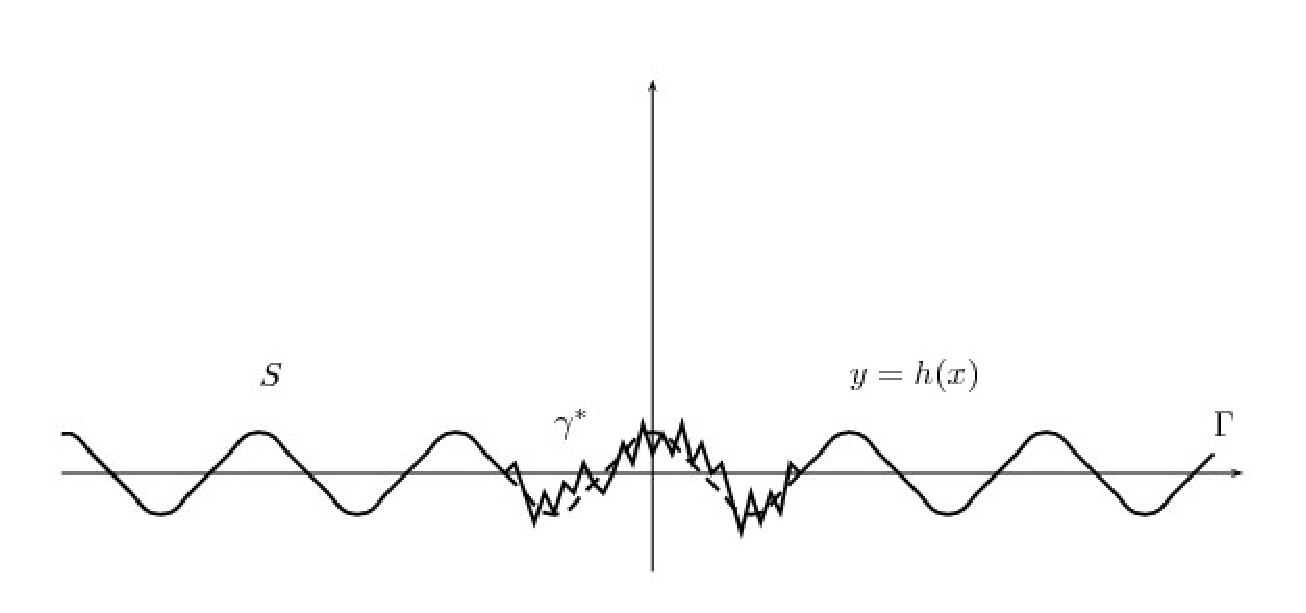
\includegraphics[width=0.85\textwidth]{deform.eps}
\captionstyle{normal}\caption{Please write your figure caption here.}\label{fig:1}
\end{figure}

The gunslinger walked stolidly, not hurrying, not loafing. A hide waterbag was slung around his middle like a bloated sausage. It was almost full. He had progressed through the khef over many years, and had reached the fifth level. At the seventh or eighth, he would not have been thirsty; he could have watched own body dehydrate with clinical, detached attention, watering its crevices and dark inner hollows only when his logic told him it must be done. He was not seventh or eighth. He was fifth. So he was thirsty, although he had no particular urge to drink. In a vague way, all this pleased him. It was romantic.

Below the waterbag were his guns, finely weighted to his hand. The two belts crisscrossed above his crotch. The holsters were oiled too deeply for even this Philistine sun to crack. The stocks of the guns were sandalwood, yellow and finely grained. The holsters were tied down with raw hide cord, and they swung heavily against his hips. The brass casings of the cartridges looped into the gun belts twinkled and flashed and heliographed in the sun. The leather made subtle creaking noises. The guns themselves made no noise. They had spilled blood. There was no need to make noise in the sterility of the desert.

\begin{multline}
\int_{a_1}^{a_2} f(x)\,dx+\int_{a_2}^{a_3} f(x)\,dx
+\dots+\int_{a_{n-1}}^{a_n} f(x)\,dx\\
+\int_{a_1}^{a_2} g(x)\,dx+\int_{a_2}^{a_3} g(x)\,dx
+\dots+\int_{a_{n-1}}^{a_n} g(x)\,dx\\
+\int_{a_1}^{a_2} h(x)\,dx+\int_{a_2}^{a_3} h(x)\,dx
+\dots+\int_{a_{n-1}}^{a_n} h(x)\,dx\\
=\int_{a_1}^{a_n} f(x)+g(x)+h(x)\,dx.
\end{multline}

His clothes were the no-color of rain or dust. His shirt was open at the throat, with a rawhide thong dangling loosely in hand-punched eyelets. His pants were seam-stretched dungarees.

He breasted a gently rising dune (although there was no sand here; the desert was hardpan, and even the harsh winds that blew when dark came raised only an aggravating harsh dust like scouring powder) and saw the kicked remains of a tiny campfire on the lee side, the side which the sun would quit earliest. Small signs like this, once more affirming the man in black?s essential humanity, never failed to please him. His lips stretched in the pitted, flaked remains of his face. He squatted.

He had burned the devil-grass, of course. It was the only thing out here that would burn. It burned with a greasy, flat light, and it burned slow. Border dwellers had told him that devils lived even in the flames. They burned it but would not look into the light. They said the devils hypnotized, beckoned, would eventually draw the one who looked into the fires. And the next man foolish enough to look into the fire might see you.

The burned grass was crisscrossed in the now-familiar ideographic pattern, and crumbled to gray senselessness before the gunslinger?s prodding hand. 

There was nothing in the remains but a charred scrap of bacon, which he ate thoughtfully. It had always been this way. The gunslinger had followed the man in black across the desert for two months now, across the endless, screamingly monotonous purgatorial wastes, and had yet to find spoor other than the hygienic sterile ideographs of the man in black?s camp fires. He had not found a can, a bottle, or a waterbag (the gunslinger had left four of those behind, like dead snake-skins).

\section{Conclusion}

The gunslinger walked stolidly, not hurrying, not loafing. A hide waterbag was slung around his middle like a bloated sausage. It was almost full. He had progressed through the khef over many years, and had reached the fifth level. At the seventh or eighth, he would not have been thirsty; he could have watched own body dehydrate with clinical, detached attention, watering its crevices and dark inner hollows only when his logic told him it must be done. He was not seventh or eighth. He was fifth. So he was thirsty, although he had no particular urge to drink. In a vague way, all this pleased him. It was romantic.

\begin{table}[!h]
\setcaptionmargin{0mm}
\onelinecaptionsfalse
\captionstyle{flushleft}
\caption{ For the insertion of tables, the table environment is used,
 the signatures to the tables are made in the same way as the captions
 for the figures. This is an example of a table whose multi-line name
 is decorated with the \textbf{caption2} package.}
\bigskip
\begin{tabular}{|c|c|c|c|c|c|c|c|}
\hline
 &$r_c$ (\AA)&$r_0$ (\AA)&$\kappa r_0$&
 &$r_c$ (\AA) &$r_0$ (\AA)&$\kappa r_0$\\
\hline
Cu& 0.800 & 14.10 & 2.550 &Sn
& 0.680 & 1.870 & 3.700 \\
Ag& 0.990 & 15.90 & 2.710 &Pb
& 0.450 & 1.930 & 3.760 \\
Au& 1.150 & 15.90 & 2.710 &Ca
& 0.750 & 2.170 & 3.560 \\
Mg& 0.490 & 17.60 & 3.200 &Sr
& 0.900 & 2.370 & 3.720 \\
Zn& 0.300 & 15.20 & 2.970 &Li
& 0.380 & 1.730 & 2.830 \\
Cd& 0.530 & 17.10 & 3.160 &Na
& 0.760 & 2.110 & 3.120 \\
Hg& 0.550 & 17.80 & 3.220 &K &  1.120 & 2.620 & 3.480 \\
Al& 0.230 & 15.80 & 3.240 &Rb & 1.330 & 2.800 & 3.590 \\
Ga& 0.310 & 16.70 & 3.330 &Cs & 1.420 & 3.030 & 3.740 \\
In& 0.460 & 18.40 & 3.500 &Ba & 0.960 & 2.460 & 3.780 \\
Tl& 0.480 & 18.90 & 3.550 & & & & \\[1mm]
\hline
\end{tabular}
\end{table}

Below the waterbag were his guns, finely weighted to his hand. The two belts crisscrossed above his crotch. The holsters were oiled too deeply for even this Philistine sun to crack. The stocks of the guns were sandalwood, yellow and finely grained. The holsters were tied down with raw hide cord, and they swung heavily against his hips. The brass casings of the cartridges looped into the gun belts twinkled and flashed and heliographed in the sun. The leather made subtle creaking noises. The guns themselves made no noise. They had spilled blood. There was no need to make noise in the sterility of the desert.

His clothes were the no-color of rain or dust. His shirt was open at the throat, with a rawhide thong dangling loosely in hand-punched eyelets. His pants were seam-stretched dungarees.

\begin{acknowledgments}
We thank A.~A.~Surname1 and B.~B.~Surname2 for their participation in discussions of the results. We are grateful to C.~C.~Surname3 and the reviewers for careful reading of the manuscript and helpful remarks. Links to grants are also listed here.
\end{acknowledgments}

\begin{thebibliography}{99}

\bibitem{ex}
\refitem{article}
Doerfler D., Deslippe J., Williams S. et al., \textquotedblleft Applying the Roofline Performance Model to the Intel Xeon Phi Knights Landing Processor. ,\textquotedblright M. Taufer et al. (Eds.): ISC High Performance Workshops 2016, LNCS. - 2016. - vol. 9945. - pp. 339?353. DOI: 10.1007/978-3-319-46079-6.

\bibitem{ex}
\refitem{article}
Doerfler D., Deslippe J., Williams S. et al., \textquotedblleft Applying the Roofline Performance Model to the Intel Xeon Phi Knights Landing Processor. ,\textquotedblright M. Taufer et al. (Eds.): ISC High Performance Workshops 2016, LNCS. - 2016. - vol. 9945. - pp. 339?353. DOI: 10.1007/978-3-319-46079-6.

\bibitem{ex}
\refitem{article}
Doerfler D., Deslippe J., Williams S. et al., \textquotedblleft Applying the Roofline Performance Model to the Intel Xeon Phi Knights Landing Processor. ,\textquotedblright M. Taufer et al. (Eds.): ISC High Performance Workshops 2016, LNCS. - 2016. - vol. 9945. - pp. 339?353. DOI: 10.1007/978-3-319-46079-6.

\bibitem{ex}
\refitem{article}
Doerfler D., Deslippe J., Williams S. et al., \textquotedblleft Applying the Roofline Performance Model to the Intel Xeon Phi Knights Landing Processor. ,\textquotedblright M. Taufer et al. (Eds.): ISC High Performance Workshops 2016, LNCS. - 2016. - vol. 9945. - pp. 339?353. DOI: 10.1007/978-3-319-46079-6.

\bibitem{ex}
\refitem{article}
Doerfler D., Deslippe J., Williams S. et al., \textquotedblleft Applying the Roofline Performance Model to the Intel Xeon Phi Knights Landing Processor. ,\textquotedblright M. Taufer et al. (Eds.): ISC High Performance Workshops 2016, LNCS. - 2016. - vol. 9945. - pp. 339?353. DOI: 10.1007/978-3-319-46079-6.

\bibitem{ex}
\refitem{article}
Doerfler D., Deslippe J., Williams S. et al., \textquotedblleft Applying the Roofline Performance Model to the Intel Xeon Phi Knights Landing Processor. ,\textquotedblright M. Taufer et al. (Eds.): ISC High Performance Workshops 2016, LNCS. - 2016. - vol. 9945. - pp. 339?353. DOI: 10.1007/978-3-319-46079-6.

\bibitem{ex}
\refitem{article}
Doerfler D., Deslippe J., Williams S. et al., \textquotedblleft Applying the Roofline Performance Model to the Intel Xeon Phi Knights Landing Processor. ,\textquotedblright M. Taufer et al. (Eds.): ISC High Performance Workshops 2016, LNCS. - 2016. - vol. 9945. - pp. 339?353. DOI: 10.1007/978-3-319-46079-6.

\bibitem{ex}
\refitem{article}
Doerfler D., Deslippe J., Williams S. et al., \textquotedblleft Applying the Roofline Performance Model to the Intel Xeon Phi Knights Landing Processor. ,\textquotedblright M. Taufer et al. (Eds.): ISC High Performance Workshops 2016, LNCS. - 2016. - vol. 9945. - pp. 339?353. DOI: 10.1007/978-3-319-46079-6.

\bibitem{ex}
\refitem{article}
Doerfler D., Deslippe J., Williams S. et al., \textquotedblleft Applying the Roofline Performance Model to the Intel Xeon Phi Knights Landing Processor. ,\textquotedblright M. Taufer et al. (Eds.): ISC High Performance Workshops 2016, LNCS. - 2016. - vol. 9945. - pp. 339?353. DOI: 10.1007/978-3-319-46079-6.

\bibitem{ex}
\refitem{article}
Doerfler D., Deslippe J., Williams S. et al., \textquotedblleft Applying the Roofline Performance Model to the Intel Xeon Phi Knights Landing Processor. ,\textquotedblright M. Taufer et al. (Eds.): ISC High Performance Workshops 2016, LNCS. - 2016. - vol. 9945. - pp. 339?353. DOI: 10.1007/978-3-319-46079-6.

\bibitem{ex}
\refitem{article}
Doerfler D., Deslippe J., Williams S. et al., \textquotedblleft Applying the Roofline Performance Model to the Intel Xeon Phi Knights Landing Processor. ,\textquotedblright M. Taufer et al. (Eds.): ISC High Performance Workshops 2016, LNCS. - 2016. - vol. 9945. - pp. 339?353. DOI: 10.1007/978-3-319-46079-6.

\bibitem{ex}
\refitem{article}
Doerfler D., Deslippe J., Williams S. et al., \textquotedblleft Applying the Roofline Performance Model to the Intel Xeon Phi Knights Landing Processor. ,\textquotedblright M. Taufer et al. (Eds.): ISC High Performance Workshops 2016, LNCS. - 2016. - vol. 9945. - pp. 339?353. DOI: 10.1007/978-3-319-46079-6.

\bibitem{ex}
\refitem{article}
Doerfler D., Deslippe J., Williams S. et al., \textquotedblleft Applying the Roofline Performance Model to the Intel Xeon Phi Knights Landing Processor. ,\textquotedblright M. Taufer et al. (Eds.): ISC High Performance Workshops 2016, LNCS. - 2016. - vol. 9945. - pp. 339?353. DOI: 10.1007/978-3-319-46079-6.

\bibitem{ex}
\refitem{article}
Doerfler D., Deslippe J., Williams S. et al., \textquotedblleft Applying the Roofline Performance Model to the Intel Xeon Phi Knights Landing Processor. ,\textquotedblright M. Taufer et al. (Eds.): ISC High Performance Workshops 2016, LNCS. - 2016. - vol. 9945. - pp. 339?353. DOI: 10.1007/978-3-319-46079-6.

\bibitem{ex}
\refitem{article}
Doerfler D., Deslippe J., Williams S. et al., \textquotedblleft Applying the Roofline Performance Model to the Intel Xeon Phi Knights Landing Processor. ,\textquotedblright M. Taufer et al. (Eds.): ISC High Performance Workshops 2016, LNCS. - 2016. - vol. 9945. - pp. 339?353. DOI: 10.1007/978-3-319-46079-6.

\bibitem{ex}
\refitem{article}
Doerfler D., Deslippe J., Williams S. et al., \textquotedblleft Applying the Roofline Performance Model to the Intel Xeon Phi Knights Landing Processor. ,\textquotedblright M. Taufer et al. (Eds.): ISC High Performance Workshops 2016, LNCS. - 2016. - vol. 9945. - pp. 339?353. DOI: 10.1007/978-3-319-46079-6.

\bibitem{ex}
\refitem{article}
Doerfler D., Deslippe J., Williams S. et al., \textquotedblleft Applying the Roofline Performance Model to the Intel Xeon Phi Knights Landing Processor. ,\textquotedblright M. Taufer et al. (Eds.): ISC High Performance Workshops 2016, LNCS. - 2016. - vol. 9945. - pp. 339?353. DOI: 10.1007/978-3-319-46079-6.

\bibitem{ex}
\refitem{article}
Doerfler D., Deslippe J., Williams S. et al., \textquotedblleft Applying the Roofline Performance Model to the Intel Xeon Phi Knights Landing Processor. ,\textquotedblright M. Taufer et al. (Eds.): ISC High Performance Workshops 2016, LNCS. - 2016. - vol. 9945. - pp. 339?353. DOI: 10.1007/978-3-319-46079-6.

\bibitem{ex}
\refitem{article}
Doerfler D., Deslippe J., Williams S. et al., \textquotedblleft Applying the Roofline Performance Model to the Intel Xeon Phi Knights Landing Processor. ,\textquotedblright M. Taufer et al. (Eds.): ISC High Performance Workshops 2016, LNCS. - 2016. - vol. 9945. - pp. 339?353. DOI: 10.1007/978-3-319-46079-6.

\bibitem{ex}
\refitem{article}
Doerfler D., Deslippe J., Williams S. et al., \textquotedblleft Applying the Roofline Performance Model to the Intel Xeon Phi Knights Landing Processor. ,\textquotedblright M. Taufer et al. (Eds.): ISC High Performance Workshops 2016, LNCS. - 2016. - vol. 9945. - pp. 339?353. DOI: 10.1007/978-3-319-46079-6.

\bibitem{ex}
\refitem{article}
Doerfler D., Deslippe J., Williams S. et al., \textquotedblleft Applying the Roofline Performance Model to the Intel Xeon Phi Knights Landing Processor. ,\textquotedblright M. Taufer et al. (Eds.): ISC High Performance Workshops 2016, LNCS. - 2016. - vol. 9945. - pp. 339?353. DOI: 10.1007/978-3-319-46079-6.

\bibitem{ex}
\refitem{article}
Doerfler D., Deslippe J., Williams S. et al., \textquotedblleft Applying the Roofline Performance Model to the Intel Xeon Phi Knights Landing Processor. ,\textquotedblright M. Taufer et al. (Eds.): ISC High Performance Workshops 2016, LNCS. - 2016. - vol. 9945. - pp. 339?353. DOI: 10.1007/978-3-319-46079-6.

\bibitem{ex}
\refitem{article}
Doerfler D., Deslippe J., Williams S. et al., \textquotedblleft Applying the Roofline Performance Model to the Intel Xeon Phi Knights Landing Processor. ,\textquotedblright M. Taufer et al. (Eds.): ISC High Performance Workshops 2016, LNCS. - 2016. - vol. 9945. - pp. 339?353. DOI: 10.1007/978-3-319-46079-6.

\bibitem{ex}
\refitem{article}
Doerfler D., Deslippe J., Williams S. et al., \textquotedblleft Applying the Roofline Performance Model to the Intel Xeon Phi Knights Landing Processor. ,\textquotedblright M. Taufer et al. (Eds.): ISC High Performance Workshops 2016, LNCS. - 2016. - vol. 9945. - pp. 339?353. DOI: 10.1007/978-3-319-46079-6.

\bibitem{ex}
\refitem{article}
Doerfler D., Deslippe J., Williams S. et al., \textquotedblleft Applying the Roofline Performance Model to the Intel Xeon Phi Knights Landing Processor. ,\textquotedblright M. Taufer et al. (Eds.): ISC High Performance Workshops 2016, LNCS. - 2016. - vol. 9945. - pp. 339?353. DOI: 10.1007/978-3-319-46079-6.

\bibitem{ex}
\refitem{article}
Doerfler D., Deslippe J., Williams S. et al., \textquotedblleft Applying the Roofline Performance Model to the Intel Xeon Phi Knights Landing Processor. ,\textquotedblright M. Taufer et al. (Eds.): ISC High Performance Workshops 2016, LNCS. - 2016. - vol. 9945. - pp. 339?353. DOI: 10.1007/978-3-319-46079-6.

\bibitem{ex}
\refitem{article}
Doerfler D., Deslippe J., Williams S. et al., \textquotedblleft Applying the Roofline Performance Model to the Intel Xeon Phi Knights Landing Processor. ,\textquotedblright M. Taufer et al. (Eds.): ISC High Performance Workshops 2016, LNCS. - 2016. - vol. 9945. - pp. 339?353. DOI: 10.1007/978-3-319-46079-6.

\bibitem{ex}
\refitem{article}
Doerfler D., Deslippe J., Williams S. et al., \textquotedblleft Applying the Roofline Performance Model to the Intel Xeon Phi Knights Landing Processor. ,\textquotedblright M. Taufer et al. (Eds.): ISC High Performance Workshops 2016, LNCS. - 2016. - vol. 9945. - pp. 339?353. DOI: 10.1007/978-3-319-46079-6.

\bibitem{ex}
\refitem{article}
Doerfler D., Deslippe J., Williams S. et al., \textquotedblleft Applying the Roofline Performance Model to the Intel Xeon Phi Knights Landing Processor. ,\textquotedblright M. Taufer et al. (Eds.): ISC High Performance Workshops 2016, LNCS. - 2016. - vol. 9945. - pp. 339?353. DOI: 10.1007/978-3-319-46079-6.

\bibitem{ex}
\refitem{article}
Doerfler D., Deslippe J., Williams S. et al., \textquotedblleft Applying the Roofline Performance Model to the Intel Xeon Phi Knights Landing Processor. ,\textquotedblright M. Taufer et al. (Eds.): ISC High Performance Workshops 2016, LNCS. - 2016. - vol. 9945. - pp. 339?353. DOI: 10.1007/978-3-319-46079-6.

\end{thebibliography}

\end{document}
